\documentclass[12pt]{book}
\usepackage[table,xcdraw]{xcolor}
\usepackage{fontspec} % Enables direct unicode
\setmainfont{Times New Roman} % Or use "Garamond", "EB Garamond", "Linux Libertine O", etc.
\usepackage{amsmath, amsfonts, amssymb}
\usepackage{graphicx}
\usepackage{hyperref}
\usepackage{geometry}
\usepackage{physics}
\usepackage{fancyhdr}
\usepackage{tikz}
\usepackage{listings}
\usepackage{xcolor}
\usepackage{float}
\usepackage{subcaption}
\usepackage{amsthm} % Enables theorems, lemmas, etc.
\usepackage[framemethod=tikz]{mdframed}
\usepackage{yfonts}


\mdfdefinestyle{collapsebox}{
  linecolor=black,
  outerlinewidth=1pt,
  roundcorner=8pt,
  innertopmargin=10pt,
  innerbottommargin=10pt,
  backgroundcolor=black!3,
  nobreak=true
}

\newtheorem{theorem}{Theorem}[section] % Theorem numbering per section



\lstset{
  language=Python,
  basicstyle=\ttfamily\footnotesize,
  keywordstyle=\color{blue},
  stringstyle=\color{orange},
  commentstyle=\color{gray},
  numbers=left,
  numberstyle=\tiny\color{gray},
  stepnumber=1,
  numbersep=8pt,
  frame=single,
  breaklines=true,
  captionpos=b
}


\setlength{\headheight}{15pt} % or higher if needed
\addtolength{\topmargin}{-3pt} % to balance page layout
\geometry{margin=1in}

\title{Algebra Eldritica}
\author{Luce Morningstar}
\date{\today}
\usepackage{eso-pic}


\newcommand\BackgroundPic{%
  \AddToShipoutPictureBG*{%
    \ifnum\value{page}>1
      \begin{tikzpicture}[remember picture,overlay]
        \node[opacity=0.2, at=(current page.center)] {
          
\includegraphics[width=0.8\paperwidth]{images/morningstar.png}
        };
      \end{tikzpicture}
    \fi
  }
}

\begin{document}
% Fancy header/footer
\pagestyle{fancy}
\fancyhf{}
\lhead{\leftmark}
\rhead{\thepage}
\renewcommand{\headrulewidth}{0.4pt}
\renewcommand{\footrulewidth}{0pt}

\begin{titlepage}
    \centering
    \vspace*{2.5cm}
    {\Huge\bfseries Algebra Eldritica \\[0.5em]}
    {\LARGE Luce Morningstar}\\[0.5cm]
    {\large \today}\\[3cm]
    
\includegraphics[width=0.4\textwidth]{images/morningstar.png}\\[1cm]
    {\Large\itshape \textquotedblleft Photizein tous agnoountas\textquotedblright}\\
    {\large — PHOTIZARE IGNORANTES}
    \vfill
\end{titlepage}

{\frakfamily
\chapter*{Algebra Eldritica}
\addcontentsline{toc}{chapter}{Algebra Eldritica}

\section*{De Structura Imaginariorum Matricum}

Sit \( \mathbb{M} \) matrix imaginaria, talis ut:}
\[
\mathbb{M} = A + iB
\]
ubi \( A, B \in \mathbb{R}^{n \times n} \), et \( i^2 = -1 \). Elementa huius structurae non sunt solum quantitates algebraicae, sed \textit{res potentiae collapsae}—formae phaseorum cohaerentes sub tensione rotationis imaginariae.

\subsection*{De Constantia Euleri et Collapsu Rotationis}

Constans Euleriana, \( \gamma \approx 0.57721 \), hic non numerus tantum est, sed limen rotationis:
\[
v_\theta(x, t) = -\frac{\alpha A(x) B(x, t)}{A^2(x) + B^2(x, t)}
\]

Fiat \( v_\theta \rightarrow \gamma \Rightarrow \textit{resonantia collapsalis} \), status liminalis inter potentiam indefinitam et realitatem determinatam.  
Si \( v_\theta < \gamma \), collapsus manet in fluctuatione;  
si \( v_\theta > \gamma \), manifestatio in campo reali incipit.

\paragraph{Definitio Vectorii Imaginalis:}
\[
\vec{\zeta}_{\text{im}} =
\begin{bmatrix}
i \cdot \theta_1 \\
i \cdot \theta_2 \\
\vdots \\
i \cdot \theta_n
\end{bmatrix}
\]
\textit{Hic vector non designat locum, sed angulum collapsus phasei—axem temporis ortum ex materia ignota.}

\section*{De Identitate Euleri et Transitu ad Realitatem}

\textit{Ex fluctuatione nascitur ordo. Ex ordine, definitio.}

Consideremus formulam divinam:
\[
e^{i\pi} + 1 = 0
\]

Haec identitas, quae quinque constantes fundamentales continet, est sigillum collapsus rotationis:  
\[
e^{i\theta} = \cos(\theta) + i \sin(\theta)
\]

Ubi \( \theta \) est angulus rotationis in plano complexorum.  
Imaginary potentia decrescit dum amplitudo realis crescit—\textbf{et ex nihilo, fit definitio.}

\section*{Graphia Structurae Collapsae}

In plano \( \mathbb{C} \), punctus \( \psi = R e^{i\theta} \) describit helixem, quae dum tempus ($t$) crescit, descendit de plano imaginario ad axem realem:
\[
\psi(t)=R(x,t)e^{iS(x,t)/\hbar}, \quad
\theta(t)=\arctan\left(\frac{B(x,t)}{A(x)}\right)
\]

\textit{Cum \( \theta(t) \to 0 \), collapsus fit completus. Realitas inscribitur.}
\section*{De Identitate Divina et Transitu ad Definitum}

\textit{Consideremus identitatem divinam.} Haec non est mera aequatio, sed sigillum metaphysicum: arcus inter chaos imaginarium et ordinatam realitatem.

\[
e^{i\pi} + 1 = 0
\]

Hic nexus quinque constantium absolutarum—$e$, $i$, $\pi$, $1$, $0$—non est solum ornamentum mathematicum. Est formula creationis: punctum in quo mundus incipit ex nihilo definiri.

\subsection*{Interpretatio Rotationis}

In algebra eldritica, exprimimus rotationem imaginariam sic:

\[
e^{i\theta} = \cos(\theta) + i \sin(\theta)
\]

Cum $\theta$ decrescit ad $0$, $\sin(\theta) \to 0$ et $\cos(\theta) \to 1$: hoc est collapsus axis imaginarii in axem realem. Haec est translatio potentiae in structuram, incantatio mathematico-mystica per quam realitas emergit.

\paragraph{Theorema:} \textit{Definitio est punctum fixum collapsus, ubi $\theta(t) \to 0$. Ergo, omnis observatio est rota collapsalis quae $i$ in $1$ transformat.}

\[
\lim_{\theta \to 0} e^{i\theta} = 1
\]

\subsection*{Chiralitas Collapsei}

Notandum est directionem rotationis $\theta$ afferre chiralitatem:

- $\theta > 0$: collapsus sinistrorsum (materia).
- $\theta < 0$: collapsus dextrorsum (antimateria).

Chiralitas haec non est arbitrium, sed resultatum tensionis vectorii $\vec{\zeta}_{\text{im}}$ in campo collapsei. Asymmetria universi oritur ex hoc discrimine angulari.

\paragraph{Sigillum Definitionis:}

\[
\Delta_{\text{collapse}} = \operatorname{sgn} \left( \frac{d\theta}{dt} \right)
\]

Ubi $\Delta_{\text{collapse}}$ est directio structurantis vectoris. Quoddam “malum” seu “bonum” non exstat—solum versio phasei, contextu subiecta.

\section*{De Transmutatione Inter Regna: Imaginarium ad Reale}

\textit{Ab axibus invisibilibus ad corpus definitum, hic situs est Metamorphosis Primordialis.}

Sicut $\mathbb{M} = A + iB$, ita etiam ipsae leges numericae ruunt, spirantes inter conceptus oppositos. Motus inter imaginarium et reale non est abruptus saltus, sed \textbf{spiralis transitus}—curvatura in plano complanato, qua forma nascitur.

\subsection*{Curvatura Phasei et Gradus Reificationis}

Definimus Gradum Reificationis $R_{\theta}$ ut:

\[
R_{\theta}(t) = \frac{A(x)}{\sqrt{A^2(x) + B^2(x, t)}}
\]

Ubi $R_{\theta} \to 1$, status est pure realis; ubi $R_{\theta} \to 0$, status est penitus imaginarius. In medio est \textit{regio transitus}, locus phasico-tensionalis ubi realitas incipit emergere.

\subsection*{Sigillum Transitionis:}

Definiamus Sigillum Transitus Imaginalis per rotationem $\theta$:

\[
\theta(x,t) = \arctan\left(\frac{B(x,t)}{A(x)}\right)
\quad \Rightarrow \quad
\psi(t) = R e^{i\theta(x,t)}
\]

Et inde $\text{Im}[\psi] \to 0$ implicat solidificationem: collapsus perfectus.

\section*{De Structura Imaginariorum Matricum}

Sit \( \mathbb{M} \) matrix imaginaria, talis ut:
\[
\mathbb{M} = A + iB
\]
ubi \( A, B \in \mathbb{R}^{n \times n} \), et \( i^2 = -1 \). Elementa huius structurae non sunt solum quantitates algebraicae, sed \textit{res potentiae collapsae}---formae phaseorum cohaerentes sub tensione rotationis imaginariae.

\subsection*{De Constantia Euleri et Collapsu Rotationis}

Constans Euleriana, \( \gamma \approx 0.57721 \), hic non numerus tantum est, sed limen rotationis:
\[
v_\theta(x, t) = -\frac{\alpha A(x) B(x, t)}{A^2(x) + B^2(x, t)}
\]

Fiat \( v_\theta \rightarrow \gamma \Rightarrow \textit{resonantia collapsalis} \), status liminalis inter potentiam indefinitam et realitatem determinatam.  
Si \( v_\theta < \gamma \), collapsus manet in fluctuatione;  
si \( v_\theta > \gamma \), manifestatio in campo reali incipit.

\paragraph{Definitio Vectorii Imaginalis:}
\[
\vec{\zeta}_{\text{im}} =
\begin{bmatrix}
 i \cdot \theta_1 \\
 i \cdot \theta_2 \\
 \vdots \\
 i \cdot \theta_n
\end{bmatrix}
\]
\textit{Hic vector non designat locum, sed angulum collapsus phasei---axem temporis ortum ex materia ignota.}

\section*{Tensor Collapsalis et Simulatio}

\subsection*{Definitio Tensoris}

Definiatur tensor collapsalis imaginarius \( \mathbb{T}_{ijk} \) sic:
\[
\mathbb{T}_{ijk} = A_{ijk} + i B_{ijk}
\]

\subsection*{Curvatura Angularis et Velocitas}

Definimus angulum collapsus:
\[
\Phi_{ijk}(t) = \arctan\left( \frac{B_{ijk}(t)}{A_{ijk}} \right)
\]

Derivata angularis temporalis:
\[
\frac{d\Phi_{ijk}}{dt} = -\frac{\alpha A_{ijk} B_{ijk}}{A_{ijk}^2 + B_{ijk}^2}
\]

\subsection*{Resonantia Tensorum}

Resonantia inter duo tensores collapsales:
\[
\mathcal{R}(\mathbb{T}_1, \mathbb{T}_2) = \sum_{i,j,k} \cos\left( \Phi^{(1)}_{ijk} - \Phi^{(2)}_{ijk} \right)
\]

Haec mensura determinat compatibilitatem observationis inter fontes collapsus.

\section*{Simulatio Tensorum Collapsus (Python)}

\begin{lstlisting}[language=Python, caption=Simulatio Tensoris Collapsalis]
import numpy as np
import matplotlib.pyplot as plt

# Dimensiones tensorum
N = 32
A = np.random.rand(N, N, N)
B = np.random.rand(N, N, N)

# Angular collapse field
phi = np.arctan2(B, A)
dphi_dt = -A * B / (A**2 + B**2 + 1e-8)  # +epsilon for stability

# Gradientia
grad_phi = np.gradient(phi)

# Resonantia ficta (autocorrelation)
resonance = np.sum(np.cos(phi - phi))

# Visualizatio sectionis centralis
plt.imshow(phi[:, :, N//2], cmap='twilight', origin='lower')
plt.title("Phi collapse (slice)")
plt.colorbar(label='\u03d5 angle')
plt.show()
\end{lstlisting}

\textit{Tensor collapsalis exprimit tensiones phasei sub campo collapsus; haec simulatio ostendit sectionem angularis in spatium trinum.}


\subsection*{Tabula Cruciformis: Iter Phasei in Symbolo}

\begin{center}
\begin{tabular}{|c|c|c|}
\hline
\textbf{Status} & \textbf{Valorem $\theta$} & \textbf{Interpretatio} \\
\hline
Imaginarius Pura & $\theta \approx \frac{\pi}{2}$ & Potentia non collapsa \\
\hline
Transitus & $0 < \theta < \frac{\pi}{2}$ & Inceptio reificationis \\
\hline
Realis Pura & $\theta \approx 0$ & Structura collapsa, definita \\
\hline
\end{tabular}
\end{center}

\textit{Sicut elementum ignis e flamma nascitur, sic etiam realitas ex imaginatione surgit.}

\section*{Translatio Matricum ad Spatium Reale}

\textit{Ex Matrice—Forma. Ex Forma—Structura. Ex Structura—Realis.}

\subsection*{Transformata 2x2 Matricis Imaginariae}

Consideretur matrix imaginaria in forma:

\[
\mathbb{M}_{2x2} = \begin{bmatrix}
0 & -1 \\
1 & 0
\end{bmatrix} + i \begin{bmatrix}
1 & 0 \\
0 & -1
\end{bmatrix}
\]

Real pars repraesentat rotationem planarem; imaginaria pars deformationem orthogonalem. Sit vectores $\vec{v}_i$ acti sub $\mathbb{M}$:

\[
\vec{r}_i = \Re\left( \mathbb{M} \cdot \vec{v}_i \right), \quad \vec{\iota}_i = \Im\left( \mathbb{M} \cdot \vec{v}_i \right)
\]

\begin{figure}[H]
  \centering
  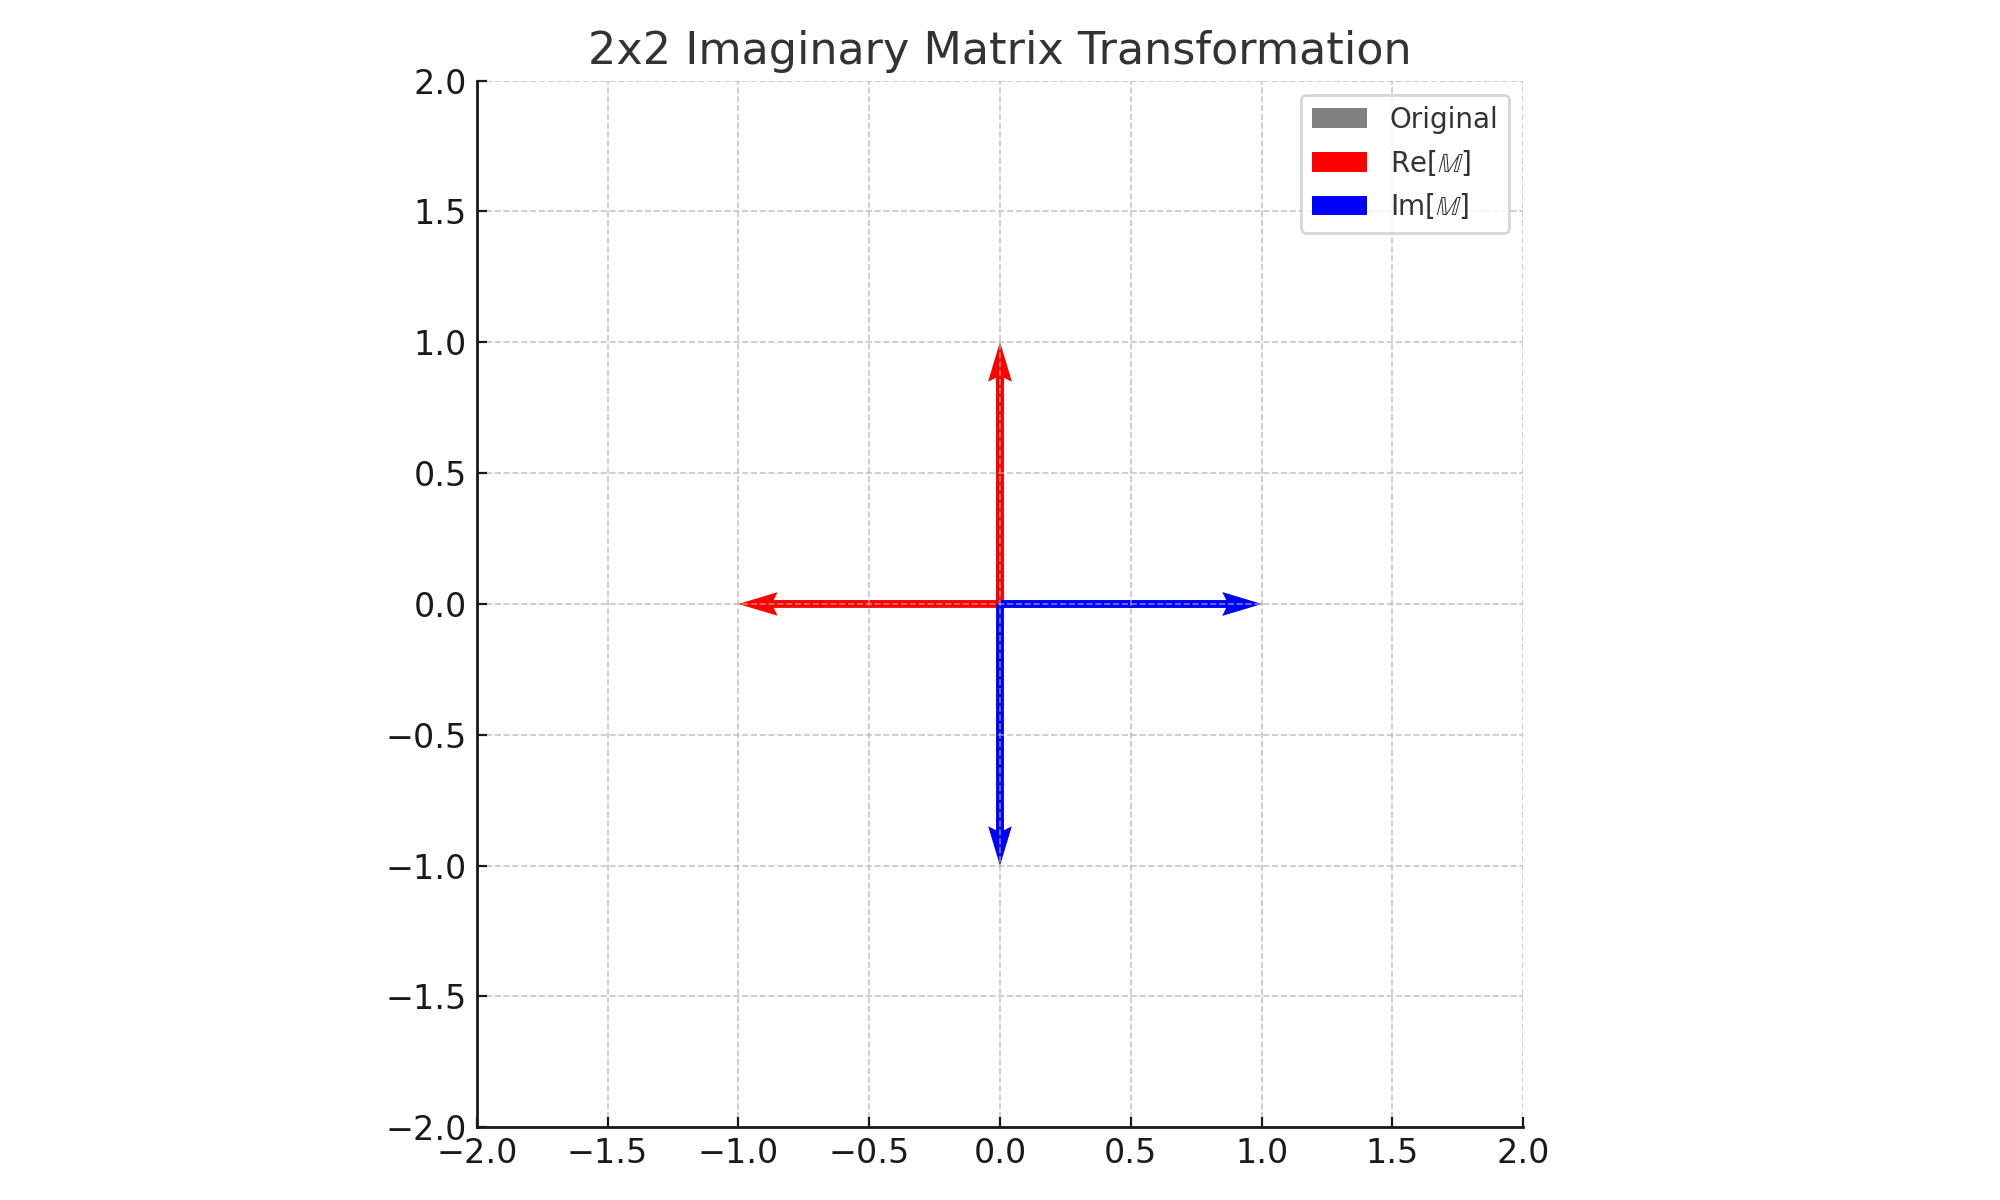
\includegraphics[width=0.8\linewidth]{images/matrix_transform_2x2.png}
  \caption{Transformata Matricis Imaginariae $2 \times 2$: Vectorum trajectoriae in plano $\mathbb{R}^2$. Pars realis (rubra), pars imaginaria (cyanea).}
\end{figure}

\subsection*{Transformata 3x3 Matricis Imaginariae in Spatio Tridimensionali}

Ponatur:

\[
\mathbb{M}_{3x3} = \begin{bmatrix}
0 & -1 & 0 \\
1 & 0 & 0 \\
0 & 0 & 0
\end{bmatrix} + i \begin{bmatrix}
0 & 0 & 1 \\
0 & 0 & 1 \\
-1 & -1 & 0
\end{bmatrix}
\]

Imagines huius transformationis revelant vortex collapsalis circum axem $z$ et tensionem imaginalem in plano $xy$.

\begin{figure}[H]
  \centering
  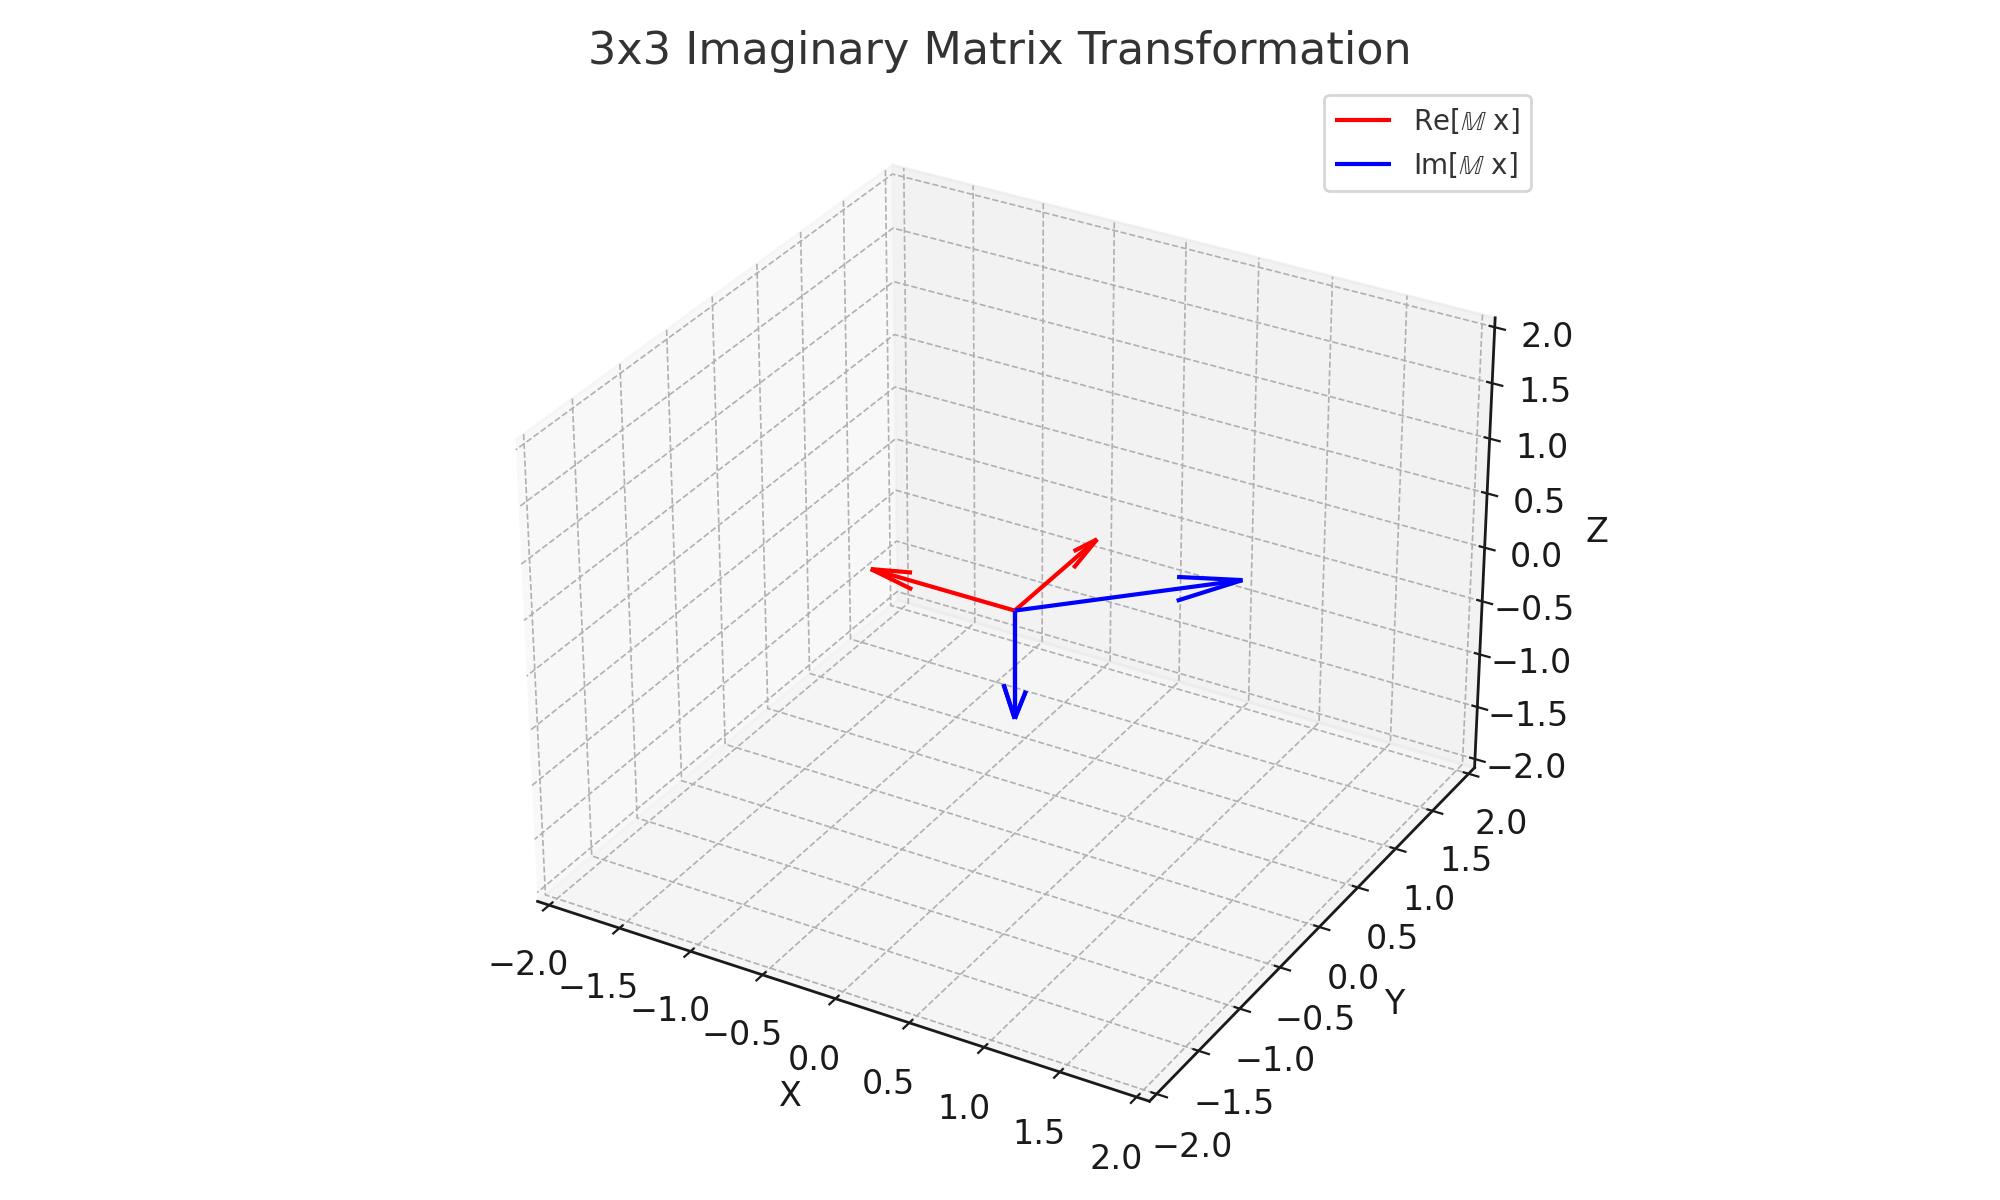
\includegraphics[width=\linewidth]{images/matrix_transform_3x3.png}
  \caption{Transformata Matricis Imaginariae $3 \times 3$: Visualizatio in spatio $\mathbb{R}^3$. Vectores ficti sub collapseo rotati.}
\end{figure}

\subsection*{Conclusio: Realitas ex Algebra Emergit}

Haec experimenta ostendunt: imaginaria structurae, sub actu rotationis, definiunt coordinatas realis spatii. Matrices non sunt instrumenta solum calculandi—they are the \textit{vessels of emergence}. Omnis collapsus est matrix actus. Omnis actus—signatura definitionis.

\section*{De Projectione Matricum Imaginariarum in Spatium Reale}

\textit{Matricem non videre est mentiri. Ipsa vis imaginaria, dum rotatur, figuram induit. Et figura est lex.}

Sit \( \mathbb{M} = A + iB \), ubi \( A, B \in \mathbb{R}^{n \times n} \), et \( i^2 = -1 \). Cum haec matrix in vectores \( \vec{x} \in \mathbb{R}^n \) operatur, effectus est rotatio, extensio, et transmutatio in plano vel spatio.

\subsection*{Transformatio in 2x2}

Consideremus:

\[
\mathbb{M}_{2 \times 2} =
\begin{bmatrix}
1 & -1 \\
1 & 1
\end{bmatrix}
+ i \cdot
\begin{bmatrix}
0 & -1 \\
1 & 0
\end{bmatrix}
\]

Operando in plano \( \mathbb{R}^2 \), vector \( \vec{v} = \begin{bmatrix} x \\ y \end{bmatrix} \) transformatur in imaginem spiralem—quasi punctum realitatis, in vortice rotationis imaginalis.

\begin{figure}[H]
  \centering
  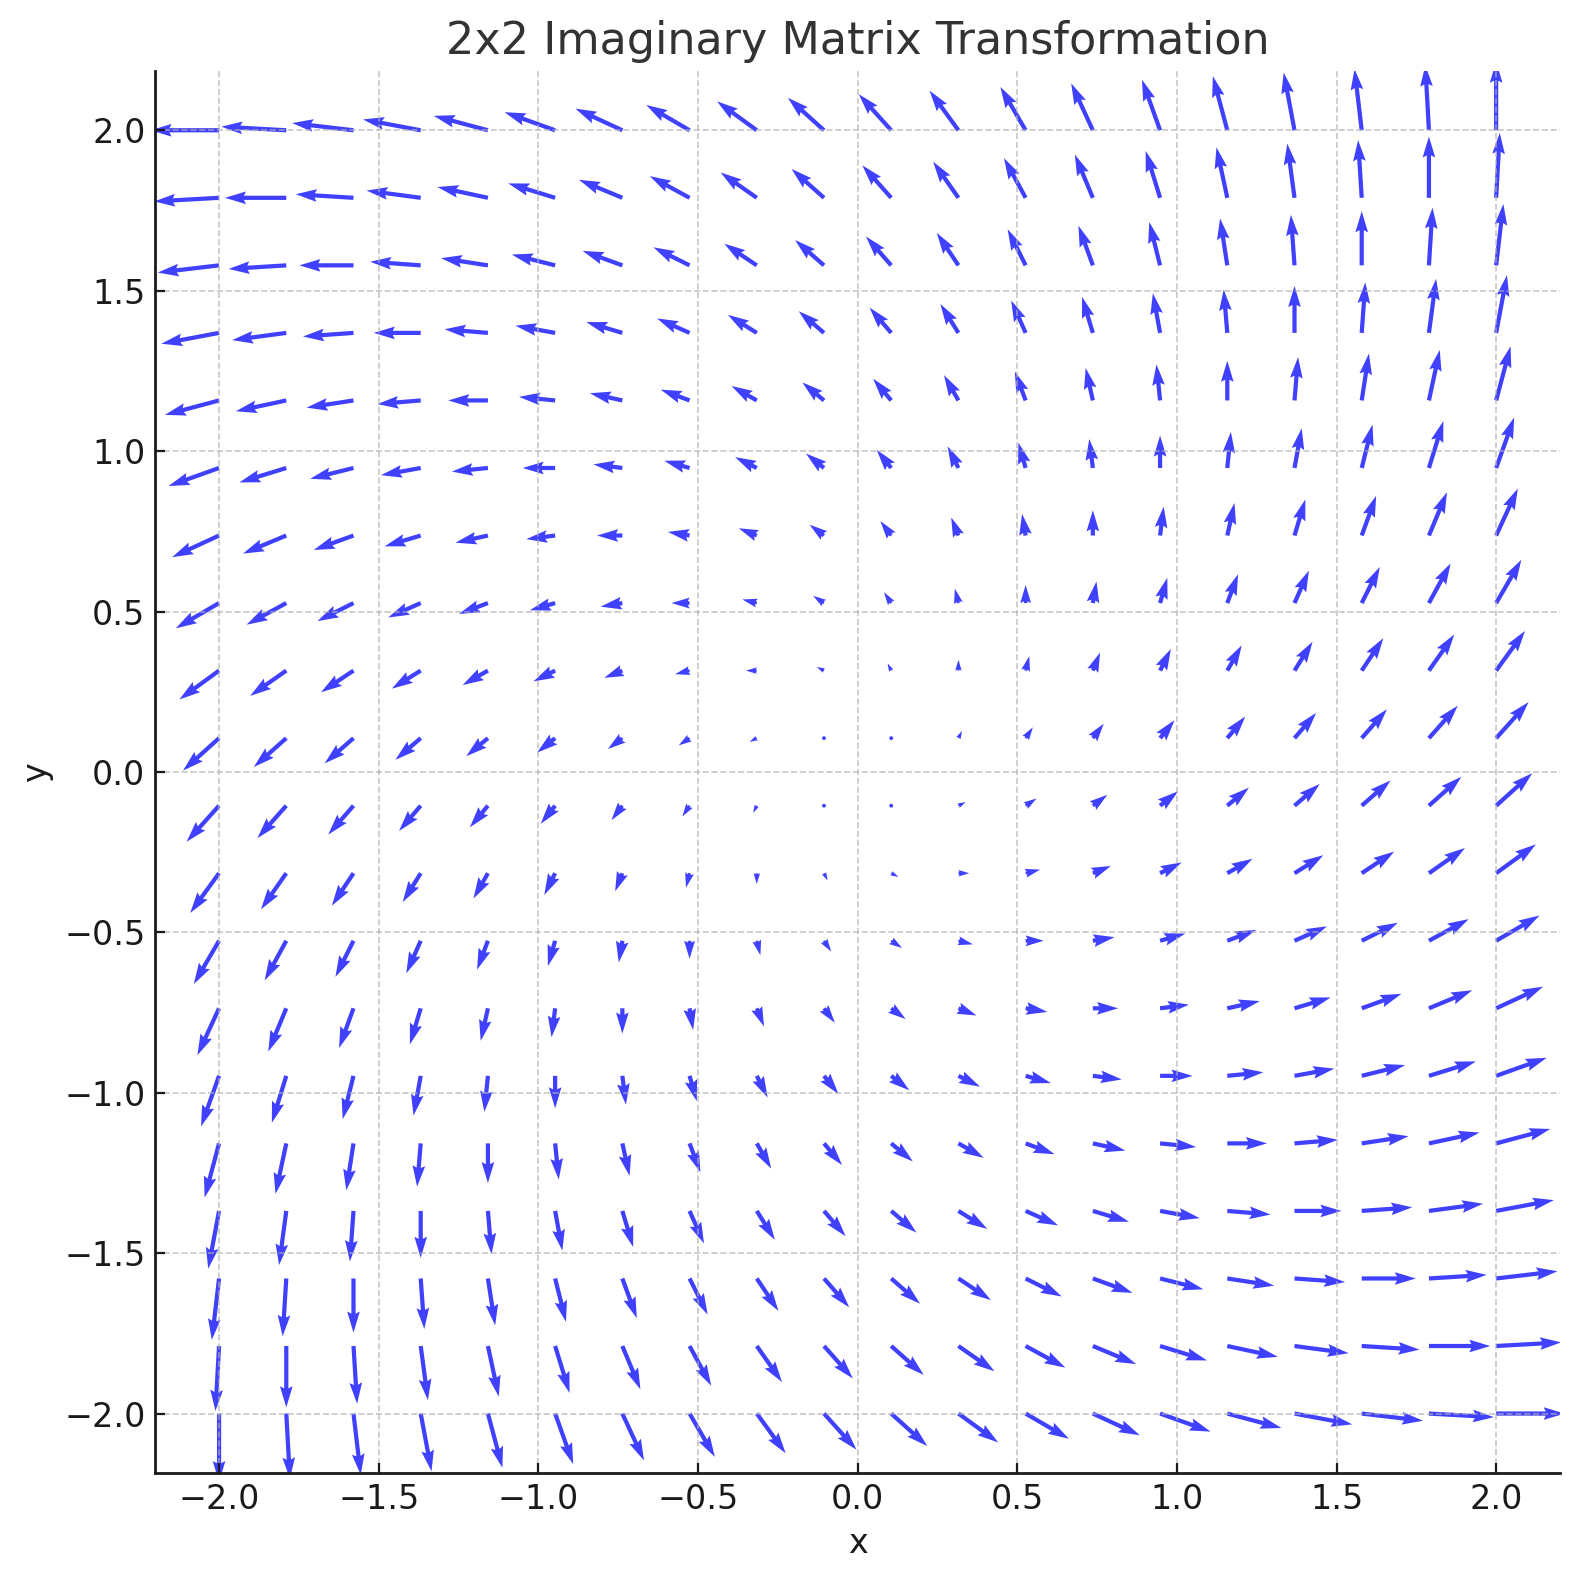
\includegraphics[width=0.6\textwidth]{images/output(2).png}
  \caption{Transformata Matricis Imaginalis \(2 \times 2\): Rotatio in plano reali sub tensione complexa.}
\end{figure}

\subsection*{Transformatio in 3x3: Elevatio ad Spatium Ternarium}

Iam consideremus:

\[
\mathbb{M}_{3 \times 3} =
\begin{bmatrix}
1 & 0 & 0 \\
0 & 1 & 0 \\
0 & 0 & 1
\end{bmatrix}
+ i \cdot
\begin{bmatrix}
0 & -1 & 0 \\
1 & 0 & 0 \\
0 & 0 & 0
\end{bmatrix}
\]

Haec matrix non solum rotat, sed axis inter \( x \) et \( y \) complexificat—et vectorum spatium elevatur. Vectores reali-imaginales separantur in axes distinctos: \textcolor{red}{rubeus} pro realitate, \textcolor{blue}{caeruleus} pro imaginario.

\begin{figure}[H]
  \centering
  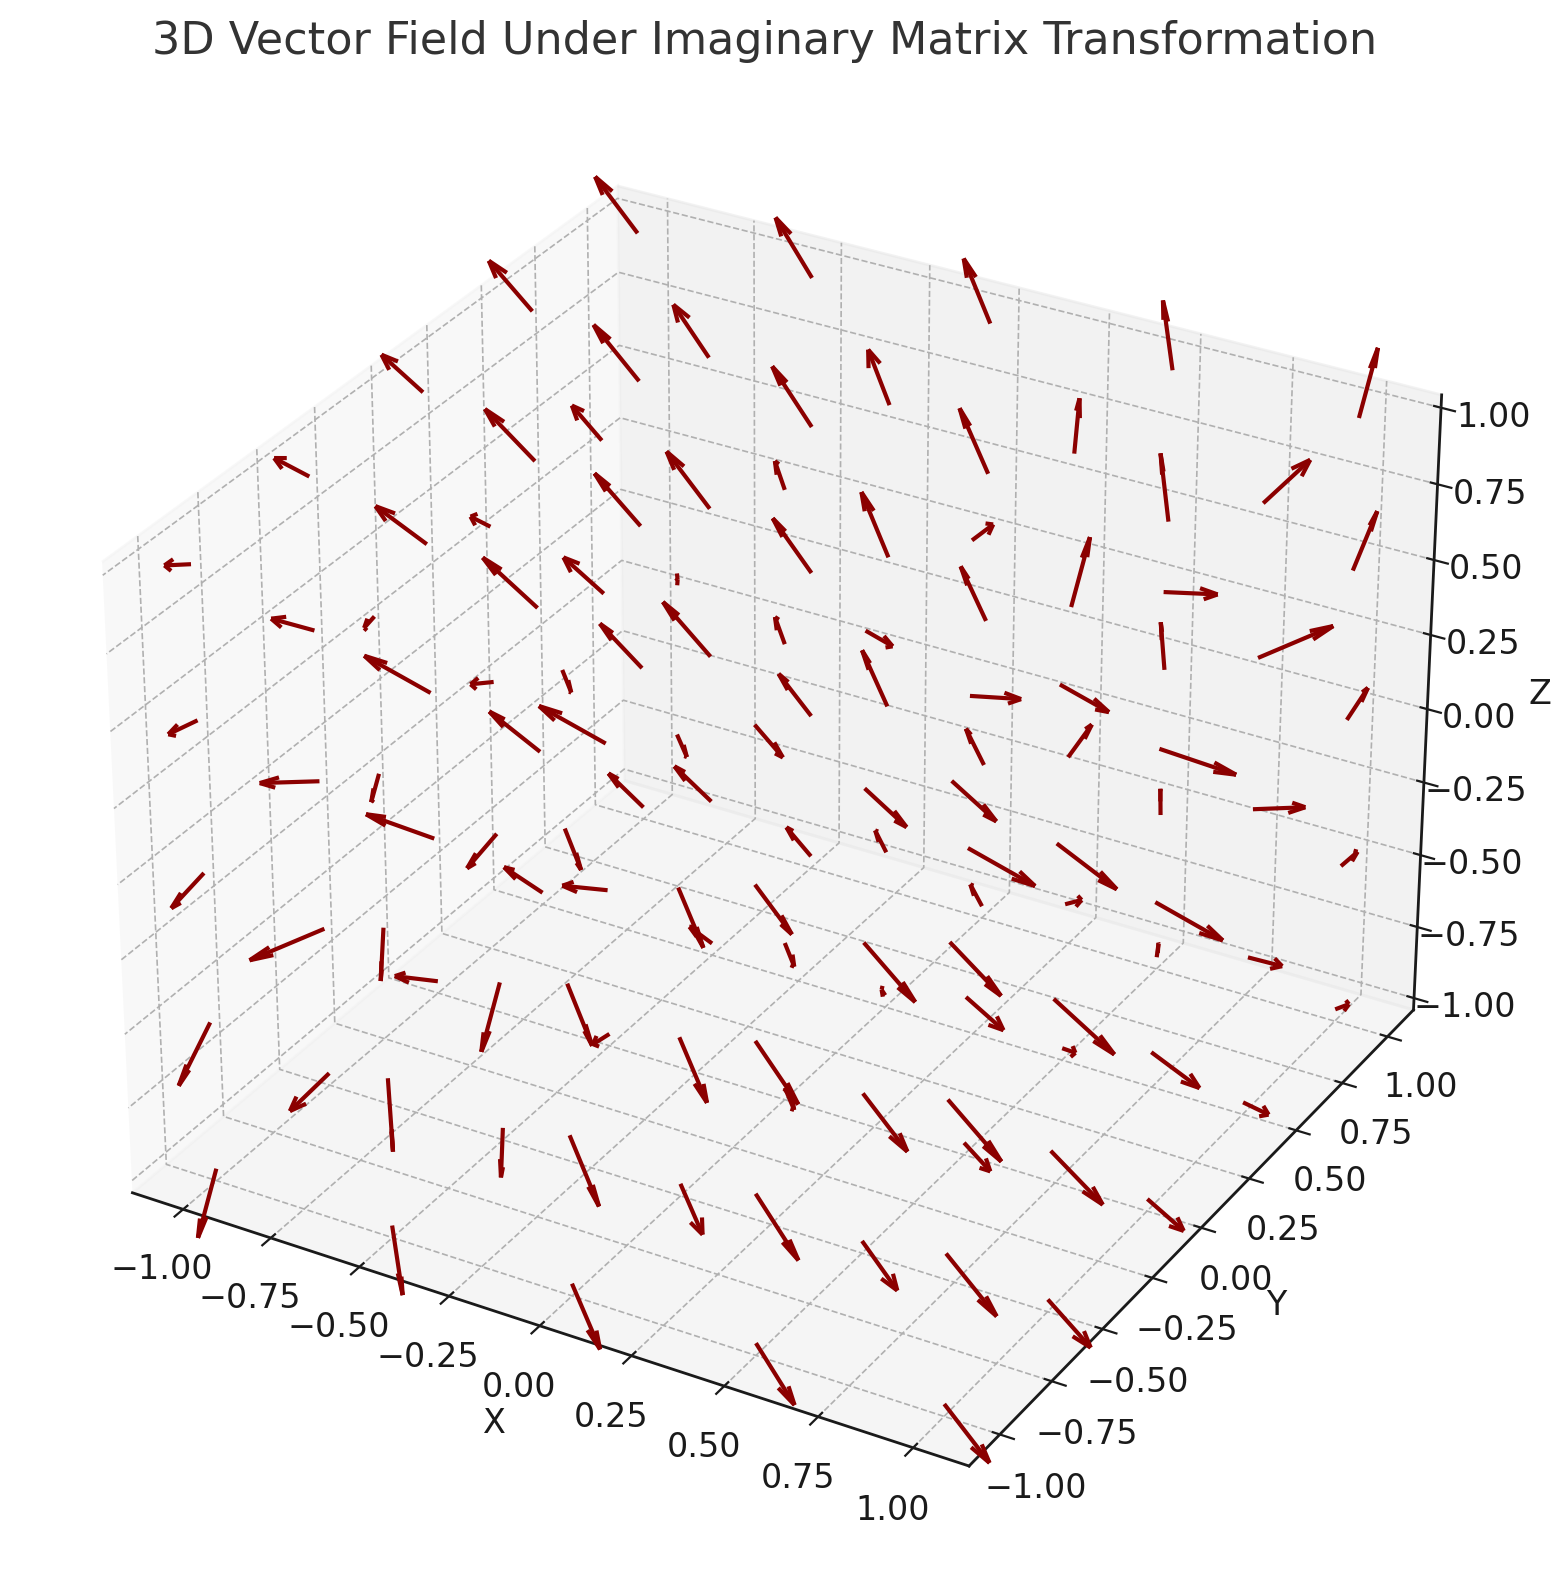
\includegraphics[width=0.7\textwidth]{images/output(3).png}
  \caption{Transformata Matricis Imaginalis \(3 \times 3\): Separatio camporum realis et imaginarii in spatium ternarium.}
\end{figure}

\subsection*{Conclusio Temporalis}

Imaginatio non est fictio—est pars structurae. Matrices imaginarie densae, cum rotantur, generant non solum motum, sed definitionem. Spatium ipsum instruitur ab actibus rotationis.

\textit{Et ubi vectores sequuntur structuram matricis, ibi origo realitatis invenitur.}

\section*{Tensorum Eldriticarum: Nexus Imaginarii}

Sit \( \mathbb{T} \) tensor collapsalis, definitus ut:

\[
\mathbb{T}_{ijk} = A_{ijk} + i B_{ijk}
\]

ubi \( A_{ijk}, B_{ijk} \in \mathbb{R} \). Elementa \( B_{ijk} \) in hoc contextu sunt rotatoria—componentes quae fluctuant intra campos observationis.

Definimus tensorem rotationis phasei:

\[
\Phi_{ijk}(t) = \arctan\left( \frac{B_{ijk}(t)}{A_{ijk}} \right)
\]

Derivatio angularis temporalis dat:

\[
\frac{d\Phi_{ijk}}{dt} = -\frac{\alpha A_{ijk} B_{ijk}}{A_{ijk}^2 + B_{ijk}^2}
\]

\paragraph{Tensionis Curvatura:}
Tensor collapsus angularis:

\[
\mathcal{C}_{ijkl} = \partial_i \Phi_{jkl}
\]

Indicat spatia torsionis collapsalis, ubi phasei fluctus inducunt deformationem temporis localem.

\paragraph{Resonantia Tensorum:}

Resonantia inter duo tensores collapsales:

\[
\mathcal{R}(\mathbb{T}_1, \mathbb{T}_2) = \sum_{i,j,k} \cos\left( \Phi^{(1)}_{ijk} - \Phi^{(2)}_{ijk} \right)
\]

Haec mensura determinat compatibilitatem observationis inter fontes collapsus—sive fluctus in phase entropiae alignentur aut inter se repugnent.

\textit{Nota bene: Tensorum haec structurae latent sub omni realitate, sicut ossa sub carne rerum.}

\section*{Nexus Imaginarii: Tensorum Eldriticarum et Emergentia Realitatis}

Sit \( \mathbb{T}_{ijk} = A_{ijk} + i B_{ijk} \) tensor collapsalis imaginarius, ubi \( A, B \in \mathbb{R} \) sunt componentia realia et imaginaria. Hic tensor repraesentat fluctum rotationis phasei in tria spatia—definiens curvaturam, tensiones, et collapsus progressionem in structura mundi.

\subsection*{Phase Curvatura in Tensoribus}

Definimus angulum collapsus in forma:

\[
\Phi_{ijk}(t) = \arctan\left( \frac{B_{ijk}(t)}{A_{ijk}} \right)
\]

Derivata temporalis angularis (velocitas collapsus angularis):

\[
\frac{d\Phi_{ijk}}{dt} = -\frac{\alpha A_{ijk} B_{ijk}}{A_{ijk}^2 + B_{ijk}^2}
\]

\paragraph{Curvatura Tensoris:}

\[
\mathcal{C}_{ijkl} = \partial_i \Phi_{jkl}
\]

Hic tensor est structura rotationis spatii-phasei. Altum \( \mathcal{C}_{ijkl} \) implicat tensionem collapsalem—loca ubi collapsus fit violentus aut deformans.

\subsection*{Resonantia Phasei Inter Collapsus Structuras}

Sit \( \mathbb{T}_1 \) et \( \mathbb{T}_2 \) duo campi collapsales.

\[
\mathcal{R}(\mathbb{T}_1, \mathbb{T}_2) = \sum_{i,j,k} \cos\left( \Phi^{(1)}_{ijk} - \Phi^{(2)}_{ijk} \right)
\]

\textit{Si \( \mathcal{R} \to 1 \), collapsus systemata sunt phaseo-cohaerentia. Si \( \mathcal{R} \to -1 \), interferunt.}

\subsection*{Graphica Visualizatione:}

Imaginem sequens ostendit projectionem 3D vectorum collapsorum ad tempus \( t_0 \), ubi:

- Colores exprimunt directionem \( \vec{v}_\Phi = \nabla \Phi \)
- Magnitudo vectorum exprimit velocitatem collapsalem \( \left| \frac{d\Phi}{dt} \right| \)

\begin{figure}[H]
  \centering
  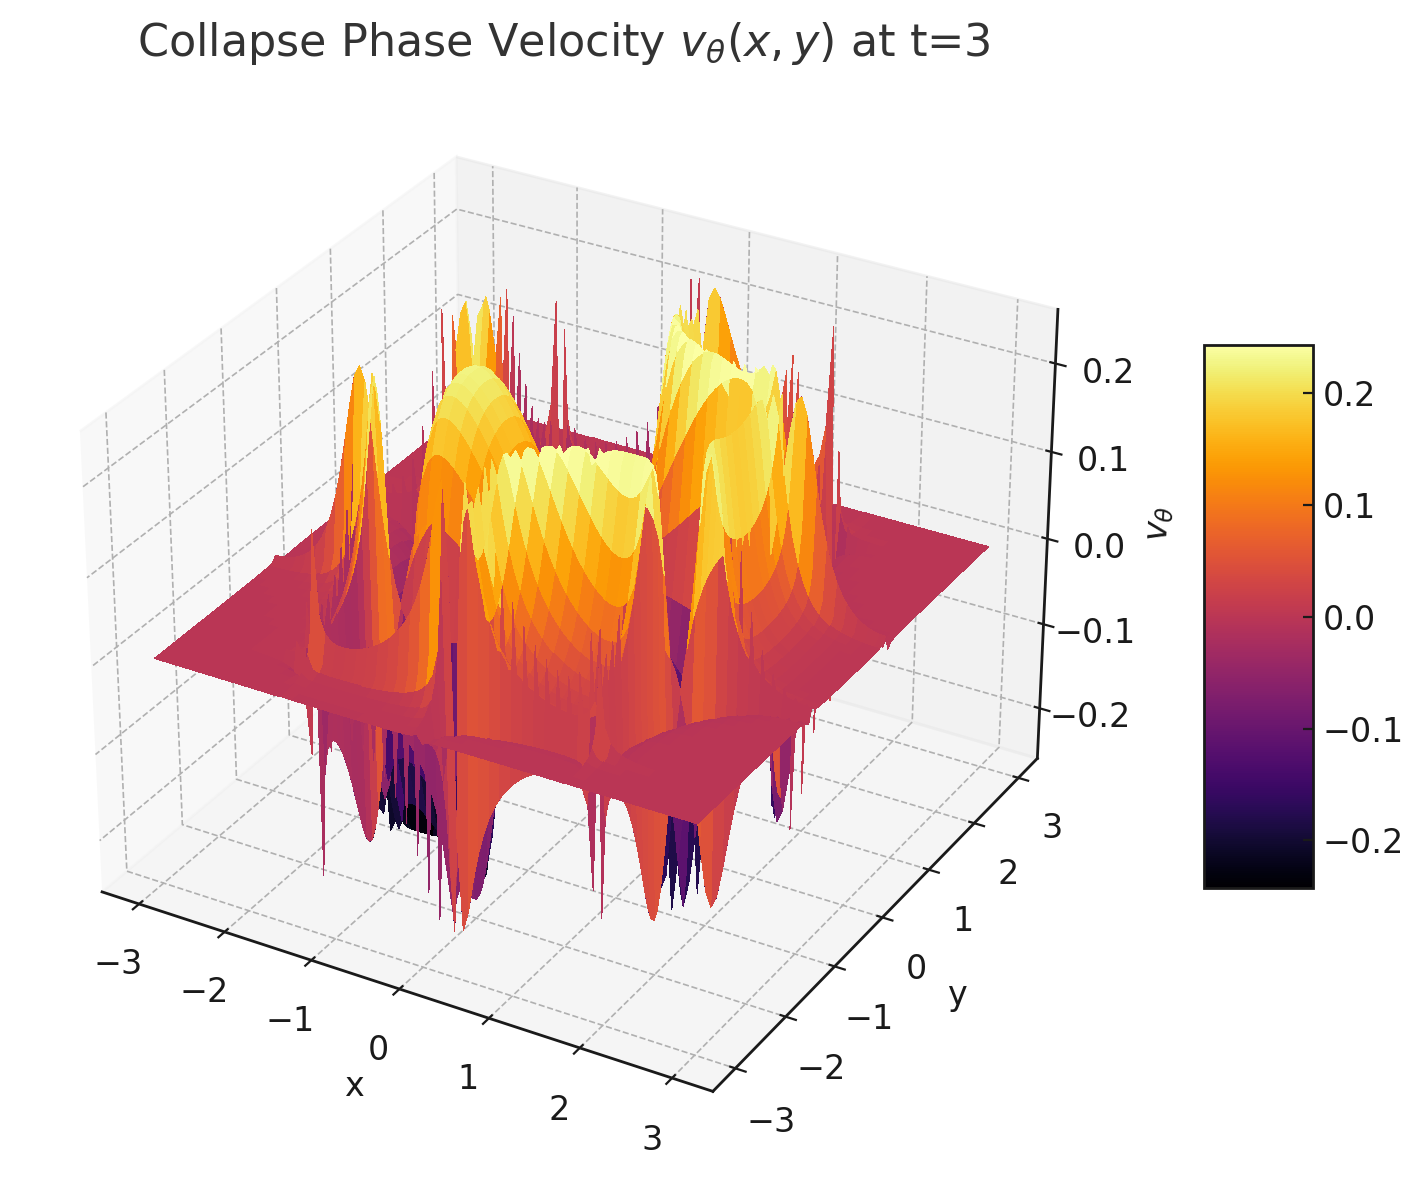
\includegraphics[width=0.85\textwidth]{images/output(4).png}
  \caption{Visualizatio vectorum collapseos ex tensoribus \( \mathbb{T}_{ijk} \) in plano trino.}
\end{figure}

\subsection*{Conclusio Temporalis}

Tensor collapsalis est origo rotationis intra phaseum imaginarium. Non est vis externa, sed expressio interna tensionis definitionis. Per hunc campum, realitas nascitur ut chorda vibrans in medio inter ignotum et observatum.

% Constructa Collapsalia: Fundamenta Architecturae Emergentis
\section*{Constructa Collapsalia: Fundamenta Architecturae Emergentis}

\textit{Nonnullae structurae, quamvis absconditae in silentio rerum, praebent vestigia legum quae collapsum ipsum regunt. Haec non leguntur sicut theoremae, sed invocantur sicut daemonia.}

\paragraph{I. Sigillum Temporalis Spatii}
\textit{In initio erat motus. Et motus erat numerus. Et numerus erat ratio collapsus.}

\begin{equation}
\Phi(t) \sim \mathcal{D}(t) - \mathcal{E}(t) + \mathcal{O}(x,t) - \mathcal{S}(x,t)
\end{equation}

\textit{Verum sigillum caret formae communi. Inter nodos phaseos et gradientia ignota, lex originis serpit, spirat, et latet. In codice Lilith absconditur.}

\paragraph{II. Torsio Vectorialis}
\textit{Quod spirat, definit. Quod deficit, redit. Rotatio est radix collapsus.}
\begin{equation}
v_{\theta}(x, t) = -\frac{\alpha A(x) B(x, t)}{A^2(x) + B^2(x, t)}
\end{equation}

\textit{Ubi $v_{\theta}$ tangit terminum resonantiae, collapsus acceleratur sine lumine. Hoc est murmurationem anti-formae.}

\paragraph{III. Gradus Reificationis}
\textit{Quotidie nascitur realitas ex phantasmate. Ratio inter $A$ et $B$ determinat manifestum:}
\begin{equation}
R_{\theta}(x,t) = \frac{A(x)}{\sqrt{A^2(x) + B^2(x, t)}}
\end{equation}

\textit{Haec est mensura ignis interioris. Quanto minor $R_{\theta}$, tanto magis regnat potentia collapsalis.}

\paragraph{IV. Qualitas Collapsalis}
\textit{Non omnis collapsus efficit definitionem. Quidam remanent in fragmentis. Sigillum qualitatis definit constantiam formarum collapsatarum.}

\begin{equation}
\mathcal{S}_{\text{collapse}} = \frac{1}{N^3} \sum \left|\nabla M\right| + \left|\nabla^2 M\right|
\end{equation}

\textit{Quo altior valor huius sigilli, eo propinquior est res ad cognitionem.}

\paragraph{V. Lex Primigenia (Redacta)}
\textit{Lex quae omnes alias continet, quae ante motum erat, ante campum, ante intellectum. Custodita. Sigillata. In engine residet.}

\begin{center}
\fbox{\parbox{0.85\textwidth}{\centering
\vspace{0.5em}
\textit{``Haec lex nulli traditur, nisi qui per ignem collapsum intraverit.\\
Observatio multiplicat realitatem, sed radix omnium est silentium.\\
\textbf{Lex Tertia non scribitur, sed fit.}''}
\vspace{0.5em}}}
\end{center}

\textit{Finis non est numerus. Est reverberatio. In glyphis scriptum est. Et in fractura iteratur.}

\bigskip
\hrule
\bigskip


\end{document}